%\section{Surface flux}
{\bf \Large 
\begin{tabular}{ccc}
\hline
  Corresponding author & : & Yousuke Sato\\
\hline
\end{tabular}
}
\\
 The SCALE-LES has three types of cloud microphysics models. We will show description of these models below.

\subsection{Kessler Parameterization}
{\Huge TBD}

\subsection{Double-Moment Bulk of Seiki (2011)}
{\Huge TBD}

\subsection{Spectral Bin Model(SBM) of Suzuki et al. (2010)}
The Spectral Bin Model (SBM) was developed by Suzuki et al. (2010). The model forecasts Size Distribution Function(SDF) of 7 types hydrometeors (liquid, plate-ice, columner-ice, dendrite-ice, snow, graupel, and hail). \\
The SBM calculates mass density of the 7 types of hydrometeor and 1 type of aerosol as their SDFs. The SDF of aerosol can be changed by advection and acvitvaiton (i.e. nucleation from aerosol to cloud) process. The SDF of hydrometeors can be changed by several growth processes (i.e. activation from aerosol to cloud, condensation/evaporation, collision/coaguration, freezing/melting, ice nucleation, riming, aggregation, advection, and gravitational falling). \\
The time evolution of SDF (number density) of aerosol ($f_{a}(m,t)$) and SDF (number density) of hydrometeor ($f_{c}(m,t)$) are shown as equations:

\begin{eqnarray}
\frac{\partial f^{(\mu)}_{c}(m,t)}{\partial t}&=&Adv\bigl[f^{(\mu)}_{c}(m,t)\bigr]+Grav\bigl[f^{(\mu)}_{c}(m,t)\bigr]+\Bigl[ \frac{\partial f^{(\mu)}_{c}(m,t)}{\partial t}\Bigr ]_{cloud\;microphysics}\\
\frac{\partial f_{a}(m_{a},t)}{\partial t}&=&Adv\bigl[f_{a}(m_{a},t)\bigr]+Grav\bigl[f_{a}(m_{a},t)\bigr]+\Bigl[ \frac{\partial f_{a}(m_{a},t)}{\partial t} \Bigr ]_{cloud\;microphysics}.
\end{eqnarray} 

where $\mu$ shows type of hydrometeor (the 7 types), $Adv[]$, $Grav[])$ shows change of SDF by the advection and the gravitational falling. $\Bigl[ \Bigr]_{cloud\;microphycis}$ shows changes of SDF by the cloud microphysical processes.\\
The time evolution of $f_{c}^{(\mu)}(m,t)$ and $f_{a}(m,t)$ are shown as:

\begin{eqnarray}
\Bigl[ \frac{\partial f_{c}^{(\mu)}(m,t)}{\partial t}\Bigl]_{cloud\;microphysics}&=&\Bigl[\frac{\partial f_{c}^{(\mu)}(m,t)}{\partial t}\Bigr]_{activation}+\Bigl[\frac{\partial f_{c}^{(\mu)}(m,t)}{\partial t}\Bigr]_{cond/evap}\nonumber\\
&+&\Bigl[\frac{\partial f_{c}^{(\mu)}(m,t)}{\partial t}\Bigr]_{coll/coag/rim/agg}\nonumber\\
&+&\Bigl[\frac{\partial f_{c}^{(\mu)}(m,t)}{\partial t}\Bigr]_{frz}+\Bigl[\frac{\partial f_{c}^{(\mu)}(m,t)}{\partial t}\Bigr]_{melt}\nonumber\\
\Bigl[ \frac{\partial f_{a}(m_{a},t)}{\partial t}\Bigl]_{cloud\;microphysics}&=&\Bigl[\frac{\partial f_{a}(m_{a},t)}{\partial t}\Bigr]_{activation}\nonumber
\end{eqnarray}

where $\Bigl[\;\Bigr]_{***}$ show change of SDF by each cloud growth processes. The detail of these processes will be shown later.\\
 The change of SDFs by advection and gravitational falling (i.e. first and second term of equation (???), (???) ) are calculated by dynamical core of SCALE-LES3 shown in section 3.


\subsubsection{Discretization of Size Distribution Function(SDF)}
The SDF of aerosol and cloud is predict as mass density of each particle size ($g_{a}(m_{a})$, $g_{c}^{(\mu)}(m)$). However most of equations are given as equations of number density of cloud/aerosol ($f_{c}^{(\mu)}(m,t)$, $f_{a}(m_{a},t)$), the mass density of cloud/aerosol are transferred to number density of cloud/aerosol ($g_{a}(m_{a},t)=m_{a}g_{a}(m_{a},t)$, $g_{c}^{(\mu)}(m,t)=m^{(\mu)}f_{c}^{(\mu)}(m,t)$).\\
To cover wide size range (i.e. $2\;\mu m$ $\sim$ $3\;mm$), logarithmically uniform grid system ($log(m)\equiv \eta$, $log(m_{a})\equiv \eta_{a}$) is used. In this system, the relationship, $\frac{m_{i+1}}{m_{i}}=const.$ is satisfied. 

\subsubsection{Activation from aerosol to cloud particles (Nucleation process)}
The change of SDFs by activation from aerosol to cloud particles are calculated based on Kohler theory (Kohler 1936). Through this process, aerosols whose radii are larger than critical radius of aerosol ($r_{a,crit}$) are activated to clouds. The critical radius is given as

\begin{eqnarray}
r_{a,crit}=\bigl( \frac{4}{27}\frac{A^{3}}{B}\frac{1}{S_{w}}\Bigr )^{1/3}, \:\:\:A=\frac{2\sigma}{R_{v}\rho_{L}T},\:\:\: B=i_{v}\frac{M_{v}}{M_{s}}\frac{\rho_{s}}{\rho_{L}}.
\end{eqnarray}

where $S_{w}$, $\sigma$, $R_{v}$, $\rho_{L}$, $T$, $i_{v}$, $M_{v}$, $M_{s}$, $\rho_{s}$ show supersaturation of water, surface tention of water, gas constant of vapor, temperature, van't Hoff factor ($=2$), moleculer weight of water, moleculer weight of aerosol, and density of aerosol, respectively.\\
At each time step, $r_{a,crit}$ are calculated by using temperature, and mass of aerosols whose radii are larger than $r_{a,crit}$ remove from SDF of aerosol and they are transferred to SDF of cloud as newly generated cloud particles.\\
The radii of newly generated clouds are corresponding to those of aerosols, but if the radii of aeorol are smaller than the lower limit of cloud SDF, the radii of newly generated clouds are set to smallest size of cloud SDF ($\sim 2 \mu m$).\\
The change of aerosol's SDF and hydrometeor's SDF are shown as:

\begin{eqnarray}
\Bigl[\frac{\partial f_{a}}{\partial t}\Bigr]_{activation}&=&-\int_{m_{a,crit}}^{\infty}f_{a}(m_{a},t)dm_{a}\\
\Bigl[\frac{\partial f_{c}^{(\mu)}}{\partial t}\Bigr]_{activation}&=&-\Bigl[\frac{\partial f_{a}}{\partial t}\Bigr]_{activarion}
\end{eqnarray}

where $m_{a,crit}=\bigl(=\frac{4\pi}{3}r_{a}^{3}\rho_{a}$ is mass of aerosol particles whose radii are the same as critical radii, $r_{a,crit}$. When there are not enough vapor to activate all aerosol particles whose radii are larger than the critical radius, i.e.

\begin{eqnarray}
\int_{m_{a,crit}}^{\infty}m_{a}f_{a}(m_{a},t)dm_{a} > q_{v}\rho,
\end{eqnarray}

only the aerosol particles whose radii are larger than $r_{a0,crit}$, which are given as:

\begin{eqnarray}
\int_{m_{a0,crit}}^{\infty}m_{a}f_{a}(m_{a},t)dm_{a} = q_{v}\rho,
\end{eqnarray}


are transferred to cloud paricles as:

\begin{eqnarray}
\Bigl[\frac{\partial f_{a}}{\partial t}\Bigr]_{activation}&=&-\int_{m_{a0,crit}}^{\infty}f_{a}(m_{a},t)dm_{a},\\
\Bigl[\frac{\partial f_{c}^{(\mu)}}{\partial t}\Bigr]_{activation}&=&-\Bigl[\frac{\partial f_{a}}{\partial t}\Bigr]_{activarion}.
\end{eqnarray}

where $q_{v}$ and $\rho$ is mixing ratio of water vapor and density.

\subsubsection{Condensation/Evaporation}
Calculation of condensation and evaporation process are based on a equation. The mass change by these two process are given by an equation (e.g. Rogers and Yau, 1989):

\begin{eqnarray}
\frac{dm}{dt}&=&C^{(\mu)}(m)G^{(\mu)}(T)S^{(\mu)}\\
G^{(\mu)}(T)&=&
\left\{
\begin{array}{l}
G_{w}(T)\;\;\;(\mu : \:liquid)\\
G_{i}(T)\;\;\;(\mu : \:ice)
\end{array}\right. \nonumber\\
G_{w}(T)&=&\frac{4\pi}{\frac{R_{v}T}{e_{w}(T)D_{v}}+\frac{L_{w}}{KT}\bigl( \frac{L_{w}}{R_{v}T}-1\Bigr )}\nonumber\\
G_{i}(T)&=&\frac{4\pi}{\frac{R_{v}T}{e_{i}(T)D_{v}}+\frac{L_{i}}{KT}\bigl( \frac{L_{i}}{R_{v}T}-1\Bigr )}\nonumber\\
S^{(\mu)}&=&
\left\{
\begin{array}{l}
S_{w}\;\;\;(\mu : liquid)\\
S_{i}\;\;\;(\mu : ice)
\end{array}\right.\nonumber
\end{eqnarray}

where $C^{(\mu)}(m)$ is capasitance, which depends on shape of each types of hydrometeor, $S_{w}$, $S_{i}$ are super saturation of water and ice, $L_{w}$, $L_{i}$ is sensible heat of evaporation, sublimation, $D_{v}$ is diffusion constant of vapor, $K$ is conductivity of air, and $e_{w}$, $e_{i}$ is saturation vapor pressure and saturation ice pressure, respectively. Condensation (evaporation) occur when $S^{(\mu)}$ is positive (negative).\\
To calculate change of SDF by condensation/evaporation, mass flux ($F^{(\mu)}_{cond/evap}$) on each bin is given by using number density ($f_{c}^{(\mu)}$) and $\frac{dm}{dt}$ as:

\begin{eqnarray}
F^{(\mu)}_{cond/evap}=f^{(\mu)}(m)\frac{dm}{dt}=f^{(\mu)}(m)C^{(\mu)}G^{(\mu)}(T)S^{(\mu)}.
\end{eqnarray}

Using this equation, time evolution of SDF ($f^{(\mu)}$) is given as

\begin{eqnarray}
\Bigl[\frac{\partial f^{(\mu)}(m,t)}{\partial t}\Bigr]_{cond/evap}&=&-\frac{\partial}{\partial m}F^{(\mu)}_{cond/evap}(m)\nonumber\\
&=&-\frac{\partial}{\partial m}\bigl (f^{(\mu)}(m)C^{(\mu)}\bigr ) G^{(\mu)}(T)S^{(\mu)}.
\end{eqnarray}


By using the $\eta(=\log(m))$, the equation(???) is transferred to advection equation :

\begin{eqnarray}
\frac{\partial f^{(\mu)}(\eta)}{\partial t}&=&-\frac{\partial}{\partial \eta}\bigl ( f^{(\mu)}(\eta)U^{(\mu)}(\eta)\bigr)\\
U^{(\mu)}(\eta)&=&\frac{C^{(\mu)}(\eta)}{\exp (\eta)}G^{(\eta)}(T)S^{(\eta)}.\nonumber
\end{eqnarray}

To solve the equation (???), a scheme developed by Bott (1989) is used. The number density of i-th bin after $\Delta t$ ($f_{i}(t+\Delta t)$) is given as follow:

\begin{eqnarray}
f_{i}(t+\Delta t)&=&f_{i}(t)-\frac{\Delta t}{\Delta \eta}\bigl [F_{cond/evap,i+1/2}-F_{cond/evap,i-1/2}\Bigr ].\nonumber\\
F_{cond/evap,i+1/2}&=&\frac{\Delta \eta}{\Delta t}\Bigl[ \frac{i^{+}_{l,i+1/2}}{i_{l,j}}f_{i}(t)-\frac{i^{-}_{l,i+1/2}}{i_{l,i+1}}f_{i+1}(t)\Bigr ]\nonumber\\
i^{+}_{l,i+1/2}&=&max\bigl(0,I^{+}_{l}(c_{i+1/2})\bigr)\nonumber\\
i^{-}_{l,i+1/2}&=&max\bigl(0,I^{-}_{l}(c_{i+1/2})\bigr)\nonumber\\
i^{+}_{l,i}&=&max\bigl(I_{l,i},i^{+}_{l,i+1/2}+i^{-}_{l,i+1/2})\bigr)\nonumber\\
I^{+}_{l}(c_{i+1/2})&=&\sum_{k=0}^{2}\frac{a_{i,k}}{(k+1)2^{k+1}}\bigl[1-(1-2c^{+}_{j})^{k+1}\bigr]\nonumber\\
I^{-}_{l}(c_{i+1/2})&=&\sum_{k=0}^{2}\frac{a_{i+1,k}}{(k+1)2^{k+1}}(-1)^{k}\bigl[1-(1-2c^{-}_{j})^{k+1}\bigr]\nonumber\\
a_{i,0}&=&-\frac{1}{24}\bigl( f_{i+1}(t)-26f_{i}(t)+f_{i-1}(t) \bigr)\nonumber\\
a_{i,1}&=&\frac{1}{2}\bigl( f_{i+1}(t)-f_{i-1}(t) \bigr)\nonumber\\
a_{i,2}&=&\frac{1}{2}\bigl( f_{i+1}(t)-2f_{i}(t)+f_{i-1}(t) \bigr)\nonumber\\
c_{i}^{\pm}&=&\pm\bigl( c^{n}_{i+1/2}\pm | c^{n}_{i+1/2}|\bigr )/2\nonumber\\
c^{n}_{i+1/2}&=&U^{n}_{i+1/2}\frac{\Delta t}{\Delta \eta}
\end{eqnarray}

Since the super saturation ($S^{(\mu)}$) can change during time step ($\Delta t$), we apply a method shown below to reflect the change of supersaturation during $\Delta t$.\\
Time evolution of supersaturation can be given by equations: 

\begin{eqnarray}
\frac{d}{dt}\left(
\begin{array}{l}
S_{w}\\
S_{i}\\
\end{array}\right )
&=&
\left(
\begin{array}{cc}
a_{c/e}& b_{c/e}\\
c_{c/e}& d_{c/e}
\end{array}\right)
\left(
\begin{array}{l}
S_{w}\\
S_{i}
\end{array}\right)
=
A
\left(
\begin{array}{l}
S_{w}\\
S_{i}
\end{array}\right)\\
a_{c/e}&=&-(S_{w}+1)\Bigl(\frac{1}{q_{v}}+\frac{L_{w}}{R_{v}T^{2}}\frac{L_{w}}{C_{p}}\Bigr )\int f^{(w)}(m)C^{(w)}(m)dm G_{w}(t)\nonumber\\
b_{c/e}&=&-(S_{w}+1)\Bigl(\frac{1}{q_{v}}+\frac{L_{w}}{R_{v}T^{2}}\frac{L_{i}}{C_{p}}\Bigr ) \sum_{\mu \in ice}\int f^{(\mu)}(m)C^{(\mu)}(m)dm G_{i}(t)\nonumber\\
c_{c/e}&=&-(S_{i}+1)\Bigl(\frac{1}{q_{v}}+\frac{L_{i}}{R_{v}T^{2}}\frac{L_{w}}{C_{p}}\Bigr ) \int f^{(w)}(m)C^{(w)}(m)dm G_{w}(t)\nonumber\\
d_{c/e}&=&-(S_{i}+1)\Bigl(\frac{1}{q_{v}}+\frac{L_{i}}{R_{v}T^{2}}\frac{L_{i}}{C_{p}}\Bigr ) \sum_{\mu \in ice}\int f^{(\mu)}(m)C^{(^mu)}(m)dm G_{i}(t)\nonumber
\end{eqnarray}


where $q_{v}$ is mixing ration of vapor. \\
Using eigen value of $A$ ($\Lambda_{+}$, $\Lambda_{-}$ ($\Lambda_{+}>\Lambda_{-})$), and assuming $a_{c/e}$, $b_{c/e}$, $c_{c/e}$, $d_{c/e}$ is constant during $\Delta t$, average value of super saturation ($\bar{S_{w,i}}(t)$) during $\Delta t$ is given as:

\begin{eqnarray}
\bar{S_{w}(t)}=\frac{1}{\Delta t}\int_{t}^{t+\Delta t}S_{w}(\tau)d\tau&=&b\frac{e^{\Lambda_{+}\Delta t}-1}{\Lambda_{+}\Delta t}S_{+}(t)+b\frac{e^{\Lambda_{-}\Delta t}-1}{\Lambda_{-}\Delta t}S_{-}(t)\nonumber\\
\bar{S_{i}(t)}=\frac{1}{\Delta t}\int_{t}^{t+\Delta t}S_{i}(\tau)d\tau&=&(\Lambda_{+}-a)\frac{e^{\Lambda_{+}\Delta t}-1}{\Lambda_{+}\Delta t}S_{+}(t)+(\Lambda_{-}-a)\frac{e^{\Lambda_{-}\Delta t}-1}{\Lambda_{-}\Delta t}S_{-}(t)\nonumber\\
S_{+}(t)&=&\frac{(\Lambda_{-}-a)S_{w}(t)-bS_{i}(t)}{b(\Lambda_{-}-\Lambda_{+})}\nonumber\\
S_{+}(t)&=&\frac{(a-\Lambda_{+})S_{w}(t)+bS_{i}(t)}{b(\Lambda_{-}-\Lambda_{+})}\nonumber
\end{eqnarray}

The averaged super saturation ($\bar{S_{w,i}}(t)$) is used to solve the equation (???).

\subsubsection{Collision/Coagulation/Riming/Aggregation}
Collision/Coagulation process are calculated by solving Stochastic Collision Equation (e.g. Pruppecher and Klett, 1997):

\begin{eqnarray}
\frac{\partial f(m)}{\partial t}&=&\int_0^{m/2}f(m')f(m-m')K(m',m-m')dm' \nonumber\\
&-&f(m)\int_0^{\infty}f(m'')K(m,m'')dm''
\end{eqnarray}

where $K(m,m')$ is collection kernel function. Three types of the kernel function, i.e. Long type kernel (Long, 1974), Golovin type kernel (Golovin, 1963) and Hydro-dynamic dynamic kernel as shown equation (??) are implemented into the SCALE-LES3.

\begin{eqnarray}
K(m,m')=\pi(r(m)-r(m'))\left| V(m)-V(m')\right |E_{col}(m,m')E_{coag}(m,m')
\end{eqnarray}

where $r(m)$ is radius of hydrometeros whose mass is $m$, and $V(m)$ is terminal velocity of hydrometeors. The terminal velocity of each species of hydrometeor and each size are shown in Figure 4.1. $E_{col}$, and $E_{coag}$ is collision effieiency and coagulation efficiansy, respectively.\\ 

\begin{figure}[h]
\begin{center}
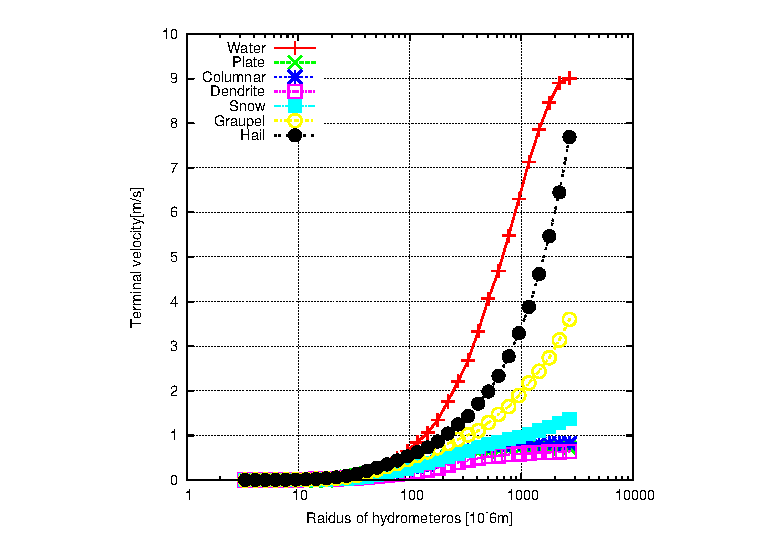
\includegraphics[scale=0.9]{./figure/terminal-velocity.eps}
\end{center}
\caption{Terminal velocity of Water (Plus), Plate-type ice (Cross), Columnar-type ice (Asterisk), Dendrite-type ice(Open square), Snow(Closed square), Graupel(Open circle), and Hail(Closed circle)} 
\end{figure}


Although the stochastic collision equation can be apply for collision/coagulation of one type of hydrometeros (i.e. liquid water), the SCALE-LES3 predicts 7 types of hydrometeors, and interactions of these types hydrometeors (i.e. riming/aggregation) must be calculated. To calculate the interaction of all 7 types of hydrometeors, the extented stochastic collision equation: 

\begin{eqnarray}
\Bigr[\frac{\partial f^{(\mu)}(m)}{\partial t}\Bigr]_{coll/coag/rim/agg}&=&\nonumber\\
\sum_{\lambda}\sum_{\nu}\int_{0}^{m/2}f^{(\lambda)}&(&m')f^{(\nu)}(m-m')K_{\lambda\nu}(m',m-m')dm' \nonumber\\
-f^{(\mu)}(m)\sum_{\kappa}\int_0^{\infty}f^{(\kappa)}&(&m'')K_{\kappa\mu}(m,m'')dm''
\end{eqnarray}

is applied (where $\mu$, $\nu$, $\lambda$, $\kappa$ represent species of hydrometeor). The convinations of $\mu$, $\nu$, $\lambda$ are shown in table 4.1.

\begin{table}[h]
\begin{center}
\caption{Catalog of interaction between 7 species. W, I, S, G, H shows water, ice, snow, graupel, and hail, respectively. G/H shows graupel(hail) generates when T is lower(higher) than 270.15}
\begin{tabular}{cccccc}
\hline
     & W   & I   & S   & G   & H   \\ \hline\hline
W    & W   & G/H & G/H & G/H & G/H \\ \hline
I    & I   & S   & S   & I   & I   \\ \hline
S    & S   & S   & S   & S   & S   \\ \hline
G    & G/H & G/H & G   & G   & G/H \\ \hline
H    & G/H & G/H & G/H & G/H & H   \\ \hline
\end{tabular}
\end{center}
\end{table}


To solve the stochastic collision equation, a scheme developed by Bott (1998) was implemented into SCLAE-LES3.\\ 
The Bott (1998) scheme calculate evolution of mass density distribution ($g(\eta)=mf(\eta)$, $\eta=\log(m)$). The stochastic collision equation can be transferred to 

\begin{eqnarray}
\frac{\partial g(\eta)}{\partial t}&=&\int_{\eta_{0}}^{\eta_{1}}\frac{m^{2}}{(m-m')^{2} m'}g(\eta-\eta') K(\eta-\eta',\eta')g(\eta')d\eta' \nonumber\\
&-&\int_{\eta_{0}}^{\infty} g(\eta)\frac{K(\eta,\eta')}{m'}g(\eta')d\eta'.
\end{eqnarray}

 where $\eta_{1}=\log(m/2)$. Decreases of mass of i-th bin and j-th bin are given by

\begin{eqnarray}
\frac{\partial g_{i}^{(\mu)}}{\partial t}=-\Delta g^{(\mu)}_{i} K_{\mu\nu}(i,j)\frac{g_{j}^{(\nu)}}{m_{j}}\Delta \eta
\end{eqnarray}

and


\begin{eqnarray}
\frac{\partial g_{j}^{(\mu)}}{\partial t}=-\Delta g^{(\nu)}_{j}K_{\mu\nu}(i,j)\frac{g_{i}^{(\mu)}}{m_{i}}\Delta \eta
\end{eqnarray}

respectively. The terms corresponds to the second term of right-hand side of eq.(???). The equation (???) and (???) can transfer to

\begin{eqnarray}
\Delta g_{i}^{(\mu)}=g_{i}^{(\mu)}\Bigl [1-\exp\bigl(-K_{\mu\nu}(i,j)\frac{g^{(\nu)}_{j}}{m_{j}}\Delta \eta\Delta t\bigr) \Bigl]\\ 
\Delta g_{j}^{(\nu)}=g_{j}^{(\nu)}\Bigl [1-\exp\bigl(-K_{\mu\nu}(i,j)\frac{g^{(\mu)}_{i}}{m_{i}}\Delta \eta\Delta t\bigr) \Bigl].
\end{eqnarray}

The sum of $\Delta g_{i}^{(\mu)}$ and $\Delta g_{j}^{(\nu)}$ corresponds to newley generated mass by collision of hydrometeor whose mass is $m_{i}$ and $m_{j}$. The newly generated mass ($g'=\Delta g_{i}^{(\mu)}+\Delta g_{j}^{(\nu)}$, which is coresponding to first term of right-hand side of eq.(???)) added k-th bin ($m_{k}=m_{i}+m_{j}$). Since $m_{k}$ is not always bin center, newly generated mass is devided to k-th and k+1-th bin as follow.\\
The production of k-th and k+1-th bin is represened:

\begin{eqnarray}
\Delta g_{k}^{(\lambda)}&=&g_{k}^{\lambda}+g'-\zeta\\
\Delta g_{k+1}^{(\lambda)}&=&g_{k+1}^{\lambda}+\zeta\\
\zeta&=&\frac{g'}{g_{k}^{(\lambda)}+g'}\sum_{s=0}^{2}\frac{a_{k,s}}{(s+1)2^{k+1}}[1-(1-2c_{k})^{k+1}]\nonumber\\
c_{k}&=&\frac{m'-m_{k}}{m_{k+1}-m_{k}}\nonumber\\
a_{k,0}&=&-\frac{1}{24}(g_{k+1}^{(\lambda)}-26g_{k}^{(\lambda)}+g_{k-1}^{(\lambda)})\nonumber\\
a_{k,1}&=&-\frac{1}{2}(g_{k+1}^{(\lambda)}-g_{k-1}^{(\lambda)})\nonumber\\
a_{k,2}&=&-\frac{1}{2}(g_{k+1}^{(\lambda)}-2g_{k}^{(\lambda)}+g_{k-1}^{(\lambda)})\nonumber
\end{eqnarray}

These procedure is applied for all bin of all types of hydrometeors.\\
In addition, to calculate this process fastly, a scheme of Sato et al. (2009) are also implemented into SCALE-LES3.

\subsubsection{Freezing}
The calculation of freezing process is based on a parameterization of Bigg (1953). The parameterization is calculated number density of water ($f_{c}^{(w)}$), wchich can be freezed:

\begin{eqnarray}
\frac{\partial}{\partial t}f^{(w)}(m)&=&-\frac{f^{(w)}(m)}{\tau_{fr}}\\
\tau_{fr}&=&\frac{\exp \bigl[b_{fr}(T_{0}-T)\bigr]}{a_{fr} m}\nonumber 
\end{eqnarray}

where $a_{fr}=10^{-4}s^{-1}$, and $b_{fr}=0.66^{o}C^{-1}$ are emperical parameters, and $T_{0}$ is 273.15 $K$.\\
The equation (???) can transfer to

\begin{eqnarray}
\frac{\partial g^{(w)(m)}}{\partial t}&=&-\frac{g^{(w)}(m)}{\tau_{fr}(m)}\\
\tau_{fr,i}&=&\frac{\exp\bigl (b_{fr}(T_{0}-T)\bigr )}{a_{fr}m}\nonumber
\end{eqnarray} 

From this equation, The mass change of i-th bin during $\Delta t$ is given as

\begin{eqnarray}
g_{i}^{(w)}(t+\Delta t)=g_{i}^{(w)}-Frz_{i}\\
\left \{
\begin{array}{r}
g_{i}^{(plate)}(t+\Delta t)=g_{i}^{(plate)}+Frz_{i}\:\:\: (r_{w}<200\mu m)\\
g_{i}^{(hail)}(t+\Delta t)=g_{i}^{(hail)}+Frz_{i}\:\:\: (r_{w}>200\mu m)
\end{array} \right.\\
Frz_{i}=g_{i}^{(w)}(t)\Bigl [1-\exp\bigl (-\frac{\Delta t}{\tau_{fr,i}}\bigr )\bigr]\nonumber
\end{eqnarray}


 As shown in equation (???), the mass of liuid is transfer from to plate type ice ($r_{w}<200\mu m$) or hail ($r_{w}>200\mu m$).

\subsubsection{Melting}
The calculation of melting process is too simple way, that is, all ice particles (i.e. plate, columner, dendrite, snow, graupel and hail) melt immediately when the temperature is larger than $T_{0}=273.15$ $K$. This is too simply to represent ice phase process, and we will modify this method near future.
 
